%
%  Vincent Yannello
%
\documentclass[12pt,fullpage]{article}
\usepackage{fullpage}
\usepackage{psfrag}                                          % LaTeX graphics tool
\usepackage{pslatex}                                         % avoids the default cmr font
\usepackage{graphicx}                                        % graphics package 
\usepackage{epsfig}                                          % figures
\usepackage{hyperref}
\usepackage{color}

\begin{document}

\noindent
{\bf Beta-binomial distribution} (from \color{blue}\url{http://www.math.wm.edu/~leemis/chart/UDR/UDR.html}\color{black})

\noindent
The shorthand $X \sim {\rm betabinomial}(a, b, n)$ is used to indicate that the
random variable $X$ has the beta-binomial distribution with parameters $a$, $b$, and $n$ where $a,b>0$ and $n$ is a positive integer.
A beta-binomial random variable $X$ with parameters $a$, $b$, and $n$ has probability mass function 
$$
f(x) = \frac{\Gamma \left( x+a \right) \Gamma \left( n-x+b \right) \Gamma \left( a+b \right)
\Gamma  \left( n+2 \right) }{ \left( n+1 \right) \Gamma  \left( a+b+n \right) \Gamma  \left( a
 \right) \Gamma  \left( b \right) \Gamma  \left( x+1 \right) \Gamma \left( n-x+1 \right)} \qquad \qquad x = 0, 1, \ldots, n.
$$
A beta-binomial random variable is a binomial random variable with a random parameter $p$ which has the
beta distribution with parameters $a$ and $b$.
The probability mass function for $n=20$ and three different parameter settings is illustrated below. \\

\begin{figure}[h!]
\begin{center}
\psfrag{labx}{$x$}
\psfrag{labf}{$f(x)$}
\psfrag{laba7}{$a = 0.7$}
\psfrag{labb2}{$b = 2$}
\psfrag{laba2}{$a = 2$}
\psfrag{laba6}{$a = 6$}
\psfrag{labb4}{$b = 4$}
\includegraphics[width=5.6in]{BetabinomialPlot.ps}
\end{center}
\end{figure}

\noindent
The cumulative distribution function, survivor function, hazard function,
cumulative hazard function, inverse distribution function, moment generating function, and characteristic function 
on the support of $X$ are mathematically intractable.

\vspace{0.05in}

\noindent
The population mean, variance, and skewness of $X$ are
$$
E[X] = \frac{na}{a+b} \qquad \qquad V[X] = \frac{nab(a+b+n)}{(a+b)^2(a+b+1)} 
$$
$$
E \left[ \left( \frac{X - \mu}{\sigma} \right)^3 \right] =
\frac{(a+b+2n)(b-a)}{(a+b+2)} \sqrt{\frac{1+a+b}{nab(n+a+b)}}.
$$
The population kurtosis of $X$ is mathematically intractable.
%
%
%\vspace{0.1in}
%
%\noindent
%{\bf APPL verification:}
%The APPL statements
%\begin{verbatim}
%assume(n, posint);
%assume(a > 0);
%assume(b > 0);
%X :=[[x->GAMMA(x+a)*GAMMA(n-x+b)*GAMMA(a+b)*GAMMA(n+2)/
%    ((n+1)*GAMMA(a+b+n)*GAMMA(a)*GAMMA(b)*GAMMA(x+1)*GAMMA(n-x+1))],
%    [0..n],["Discrete","PDF"]];
%Mean(X);
%\end{verbatim}
%verify the population mean.
%
\end{document}
